\documentclass[12pt]{article}
\usepackage{amsmath, amssymb}
\usepackage{booktabs}
\usepackage{parskip}
\usepackage[top=1in, bottom=1in, left=1in, right=1in]{geometry}
\usepackage{titling}
\usepackage{graphicx}
\usepackage{float}

\geometry{margin=1in}



\geometry{margin=1in}

\title{ODE HW 4.6}
\author{
Greyson Knippel \\[4pt]
MATH 260 --- Gonzaga University \\[4pt]
Professor Jensen \\[4pt]
\textit{Compiled with \LaTeX}
}
\date{\today}



\begin{document}

\maketitle

\section*{problem setup:}


\[
  E(t) = 12\cos(\omega t).
\]


\section*{part (a):}

\subsection*{homogeneous solution}

the homogeneous equation $I'' + 4I = 0$ has roots $r = \pm 2i$, giving
\[
  I_h = A\cos(2t) + B\sin(2t).
\]

\subsection*{particular solution}

since the forcing function is $-12\omega\sin(\omega t)$ and $\omega \neq 2$, we guess
\[
  I_p = D\sin(\omega t).
\]
substituting:
\[
  -D\omega^2\sin(\omega t) + 4D\sin(\omega t) = -12\omega\sin(\omega t)
\]
\[
  D(4 - \omega^2) = -12\omega \implies D = \frac{12\omega}{\omega^2 - 4}.
\]
so
\[
  I_p = \frac{12\omega}{\omega^2 - 4}\sin(\omega t).
\]

\subsection*{apply initial conditions}

general solution is: $I = I_h + I_p$:
\[
  I(t) = A\cos(2t) + B\sin(2t) + \frac{12\omega}{\omega^2 - 4}\sin(\omega t).
\]
from $I(0) = 0$:
\[
  A = 0.
\]
from $Q(0) = 0$, gives $I'(0) = E(0)/L = 12$:
\[
  I'(0) = 2B + \frac{12\omega^2}{\omega^2 - 4} = 12
  \implies B = \frac{12 - \frac{12\omega^2}{\omega^2-4}}{2} = \frac{-12}{\omega^2 - 4}.
\]

\subsection*{solution}

\[
  \boxed{I(t) = \frac{12}{\omega^2 - 4}\Bigl(\omega\sin(\omega t) - 2\sin(2t)\Bigr)}
\]

\begin{figure}[H]
  \centering
  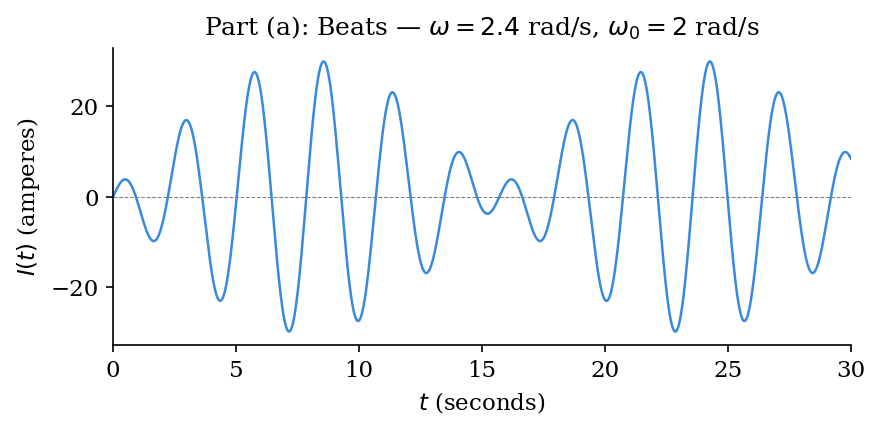
\includegraphics[width=0.85\textwidth]{plot_a.png}
  \caption{current $I(t)$ for $\omega = 2.4$ rad/s.  (made with GraphPad)}
\end{figure}

\section*{ppart (b):}


\[
  I_p = t\bigl(A\cos(2t) + B\sin(2t)\bigr).
\]
computing $I_p''$ and substituting into $I'' + 4I = -24\sin(2t)$:
\[
  -4A\sin(2t) + 4B\cos(2t) = -24\sin(2t)
  \implies A = 6,\quad B = 0.
\]
so $I_p = 6t\cos(2t)$.

general solution is:
\[
  I(t) = A\cos(2t) + B\sin(2t) + 6t\cos(2t).
\]
$I(0) = 0$ gives $A = 0$. $I'(0) = 12$ gives $B = 0$.

\subsection*{solution}

\[
  \boxed{I(t) = 6t\cos(2t)}
\]


\begin{figure}[H]
  \centering
  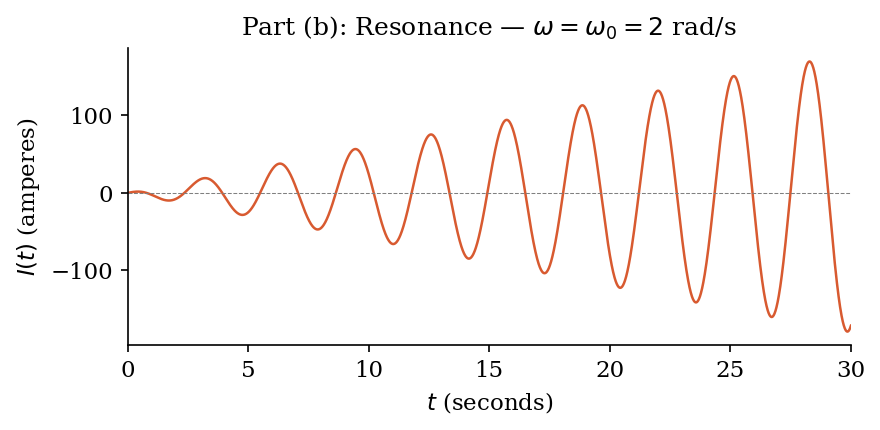
\includegraphics[width=0.85\textwidth]{plot_b.png}
  \caption{current $I(t) = 6t\cos(2t)$ at resonance. (made with GraphPad)}
\end{figure}

\end{document}